% !TeX spellcheck = en_US
% !TEX root = ../thesis-example.tex
%
\section{Additional Coloring Operations}

Finally we have created the best possible recreation of a VR actor inside the 
virtual reality scene. Now we can follow up with post effects on the video feed 
to fit it better into the environment.

\begin{figure}[htb]
	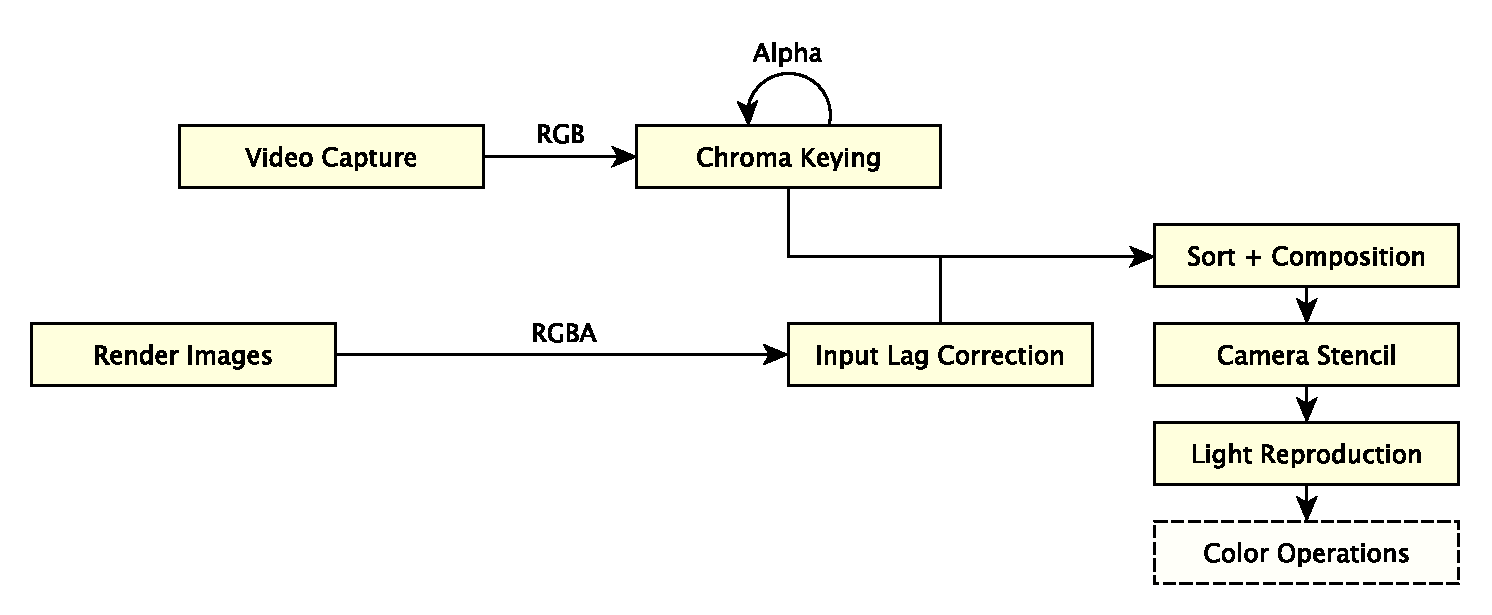
\includegraphics[width=\textwidth]{_raw_resources/pipeline_steps/4_8_color.pdf}
	\caption{Initial step upon receiving the camera image}
	\label{fig:steps:recolor}
\end{figure}

This can be done with regular coloring operations, like hue rotation, 
brightness, contrast and saturation procedures on the video alone. It gives a 
content producer direct enhancing tools which would be usually given by Unitys' 
post effects stack, which are unavailable due to the nature of this render 
pipeline.

\subsection{Color spill removal \& Recoloring}

The green box as background spills - so to say - its green color on the actor 
to a certain degree. With proper lightning setups it is possible to mitigate 
this effect but color retouching is in almost all cases a necessity. 
\textbf{YCgCo} is, again, good enough to perform this color operation, thanks 
to its color decoupling properties and a green chrominance channel. By 
splitting a RGB image into YCgCo $C_{Input}$ (see equation 
\eqref{eq:ycgco:transformation}) and then shifting towards the anti-color of a 
given key color $C_{Key}$ for a factor weight $W \in [0, 1]$:

\eq{eq:retouch:spill:1}{
	R = \frac{C_{Key Cg, Co} \cdot C_{Input Cg, Co}}{C_{Key Cg, Co} \cdot 
	C_{Key Cg, Co}}
}

\eq{eq:retouch:spill:2}{
	\begin{bmatrix}
		Y  \\
		Cg \\
		Co \\
	\end{bmatrix}
	= 
	\begin{bmatrix}
		Y \\
		C_{Key Cg} * (R + 0.5) * W \\
		C_{Key Co} * (R + 0.5) * W
	\end{bmatrix}
}

\todo{"proper lightning setup" would be something for the appendix}

Since this is a linear operation, it does not consider more apparent color 
spill around an actors edges - it slightly removes a green undertone to make 
the imagery look more natural and fitting into a scene.

Additionally we can apply a hue color rotation by using Rodrigues' rotation 
formula to make changes to the overall tint of an image, shifting a color $C_I$ 
for a maximum of 180 degrees forwards or backwards with a factor $H \in (-\pi, 
\pi]$ to yield a color $C_F$:

\eq{eq:retouch:hue}{
	C_F = C_I \cos(H) + (0.57735 \times C_I) \sin(H) + 0.57735 (k \cdot C_I) 
	(1 - \cos(H))
}
\todo{sourcing on 0.57735 needed}

With that we can achieve a more natural looking video feed that integrates well 
into any given scene. Allowing for color-shifting degrades the signal but 
allows - if needed - for a more fitting composition between an actor and his 
surrounding virtual reality scenery.

\subsection{Brightness, Contrast and Saturation}

Additionally, to give a user full control over image composition, we have a 
brief look at other linear image transformations to give good control over the 
video feed, which are brightness, contrast and saturation operations:

Brightness increases all color channels of a given color $C_I$ for a brightness 
factor of $F_B$:

\eq{eq:retouch:brightness}{
	C_T =
	\begin{bmatrix}
		C_{I_R} + F_B \\
		C_{I_G} + F_B \\
		C_{I_B} + F_B
	\end{bmatrix}
}

Contrast is a color multiplication in which the input color $C_I$ will be 
decreased by half of a channels maximum value, multiplied by a contrast factor 
$F_C$ and increased by half a maximum channels color again:

\eq{eq:retouch:contrast}{
	C_T =
	\begin{bmatrix}
		(C_{I_R} - 0.5) * F_B + 0.5 \\
		(C_{I_G} - 0.5) * F_B + 0.5 \\
		(C_{I_B} - 0.5) * F_B + 0.5
	\end{bmatrix}
}

Saturation is done by calculating the color intensity $I$ and then mixing these 
both colors for a saturation factor $F_S$:

\eq{eq:retouch:saturation:1}{
	I_{R, G, B} =
	\begin{bmatrix}
		C_{I_R} * 0.2126 \\
		C_{I_G} * 0.7152 \\
		C_{I_B} * 0.0722
	\end{bmatrix}
}

And $Lerp(x, y, t)$ being defined as:

\eq{eq:retouch:saturation:2}{
	Lerp(a, b, t) = a (1 - t) + b t
}

\eq{eq:retouch:saturation:3}{
	C_T = 
	\begin{bmatrix}
		Lerp(C_{I_R}, I_R, F_S) \\
		Lerp(C_{I_G}, I_G, F_S) \\
		Lerp(C_{I_B}, I_B, F_S)
	\end{bmatrix}
}
